\chapter{One Variable Statistics}
\section{Variables and Data}
\subsection{Definitions}

\tbf{Categorical} variables represent data that are generally grouped into categories, and are also known as qualitative variables\\

\tbf{Ordinary} variables are categorical variables whose data has a natural order but the difference between values cannot be determined
or is not meaningful\\

\tbf{Nominal} variables describe names, labels, or categories that have no natural order\\

\tbf{Quantitative} variables describe data values that are numerical, and are also known as numerical variables\\

\tbf{Continuous} variables are numerical variables which can assume an infinite number of values in a given interval\\

\tbf{Descrete} variables are numerical variables that only take on a finite number of possible values in a given interval\\

\tbf{Primary} data are data that are collected by the statisticians who are analyzing the data, from first-hand sources such as surveys or 
experiments\\

\tbf{Secondary} data are data that the statisticians who are analyzing the data did not participate in the first hand data collection 
process (ie Surveys or experiments)\\

\tbf{Microdata} contains records for each individual surveyed\\

\tbf{Aggregate} or summary data are data that are combined or summarized in such a way that the individual microdata can no longer be 
determined.\\

Data gathered from a \tbf{cross} sectional study considers individuals from different groups at the same time\\

Data gathered from a \tbf{longitudinal} study considers how the characteristics of a specific sample changes over time\\

An \tbf{index} is a continous variable such that it is an arbitrarity defined number that provides a measure of scale. 
It is used to related the values of a variable to a base level\\

The \tbf{consumer} price index, CPI, provides a broad picture of the cost of living in Canada by comparing the cost of a wide variety
of consumer goods, such as food, clothing, fuel, heating cost, transportation, shelter, and recreation\\

Health officials use the \tbf{body} mass index to determine whether a person is overweight. The BMI is calculated by dividing a person's mass
in kilograms by the square of their height in meters\\

\section{One Variable Graphs}
\subsection{Some Definitions}
A \tbf{Frequency} bar (column) graph is a visual display of data in which quantities are represented by bars of equal width, typically used with categorical or discrete data\\

A \tbf{CIRCLE} graph or \tbf{PIE} chart contains a circle divided into sectors whose areas are proportional 
to the categories represented. It is used to show how each category is compared to the whole\\

A \tbf{PICTOGRAPH} is a graph that uses pictures or symbols to represent categorical quantities. 
It's advantage is being visually appealing, hence it is the most often used graphical format. However, it may 
be difficult to present exact values when using the format, depending on the data given\\

A \textbf{STEN} and \textbf{LEAF} plot can be created easily to see the distribution of a set of numerical data.
However, its appearance is not as scientific as a histogram. \\

A \textbf{HISTOGRAM} is used to represent numerical data or data organized using intervals. The bars of a 
histogram are attached and each bar is placed between two intervals endpoints. The area of each bar is proportional
to the frequency of data in the interval. Typically, 5 ~ 15 intervals/bins of equal length are used and every piece
of data must fall into exactly one bin. The width of each bin is the \textbf{bin width} \\

Values of a continuous varialbe can be grouped into intervals in the form of \textbf{$(a, b$]} such that this interval 
includes all values from $a$ to $b$, including $a$ but excluding $b$.\\

A bin width of \textbf{5} units witht he first bin being $[10, 15)$ is reasonable if a set of continuous data 
has 26 values, a minimum of 12\\

\begin{example}

    \begin{center}
        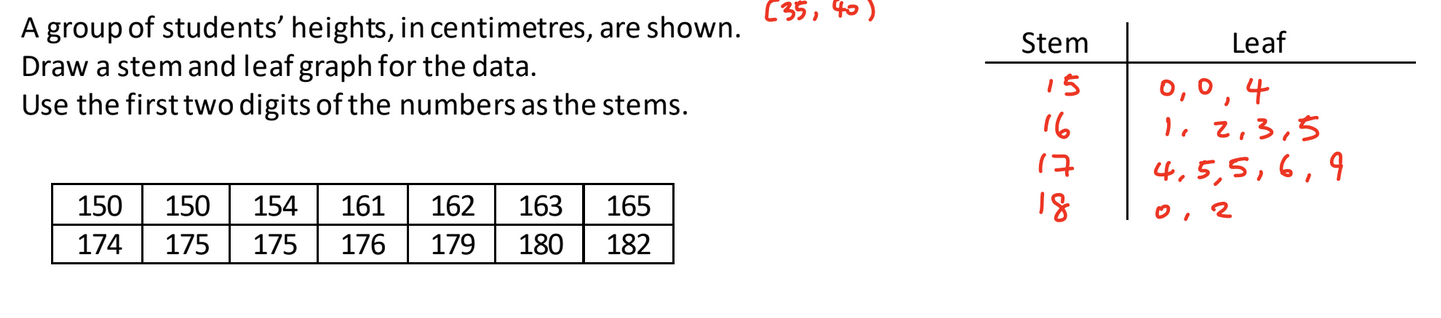
\includegraphics[width=\textwidth]{pictures/3.2.1.png}
        This is an example of \textbf{STEM and LEAF graph}
    \end{center}

\end{example}

\begin{example}
    \begin{center}
    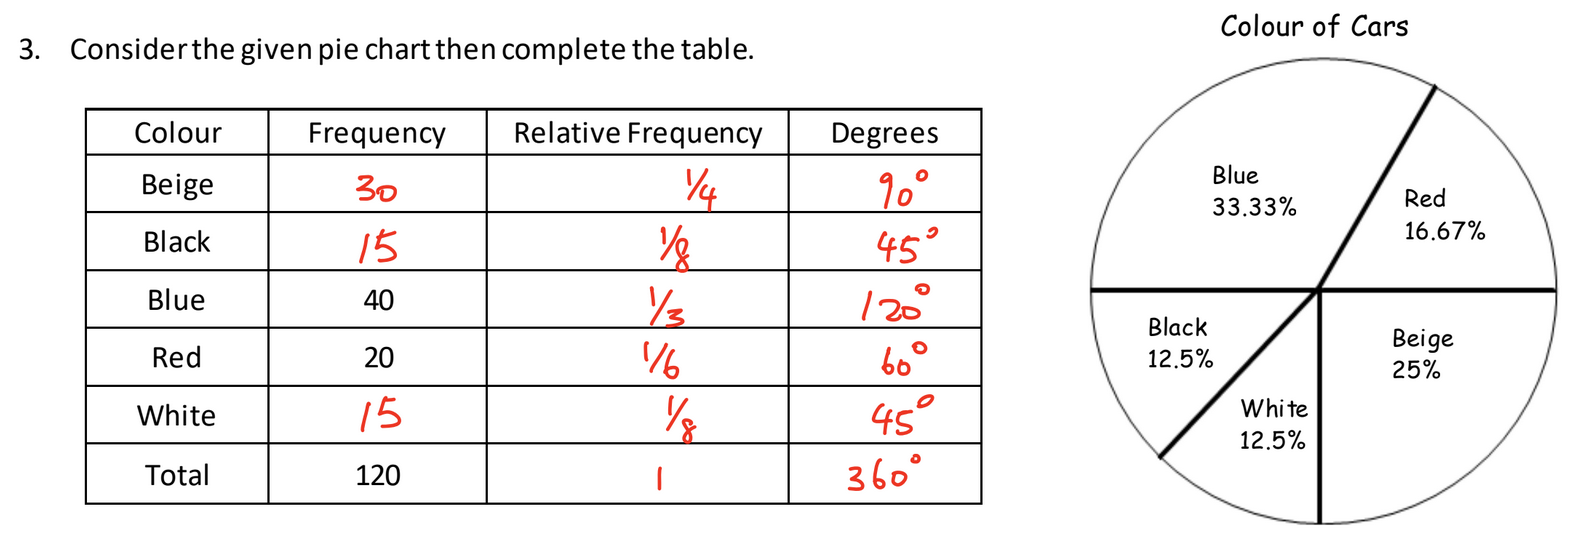
\includegraphics[width=1\textwidth]{pictures/3.2.2.png}
    \textbf{This is an Example of PIE Graphs}
    \end{center}
\end{example}
\newpage
\begin{figure}[h!]
\centering
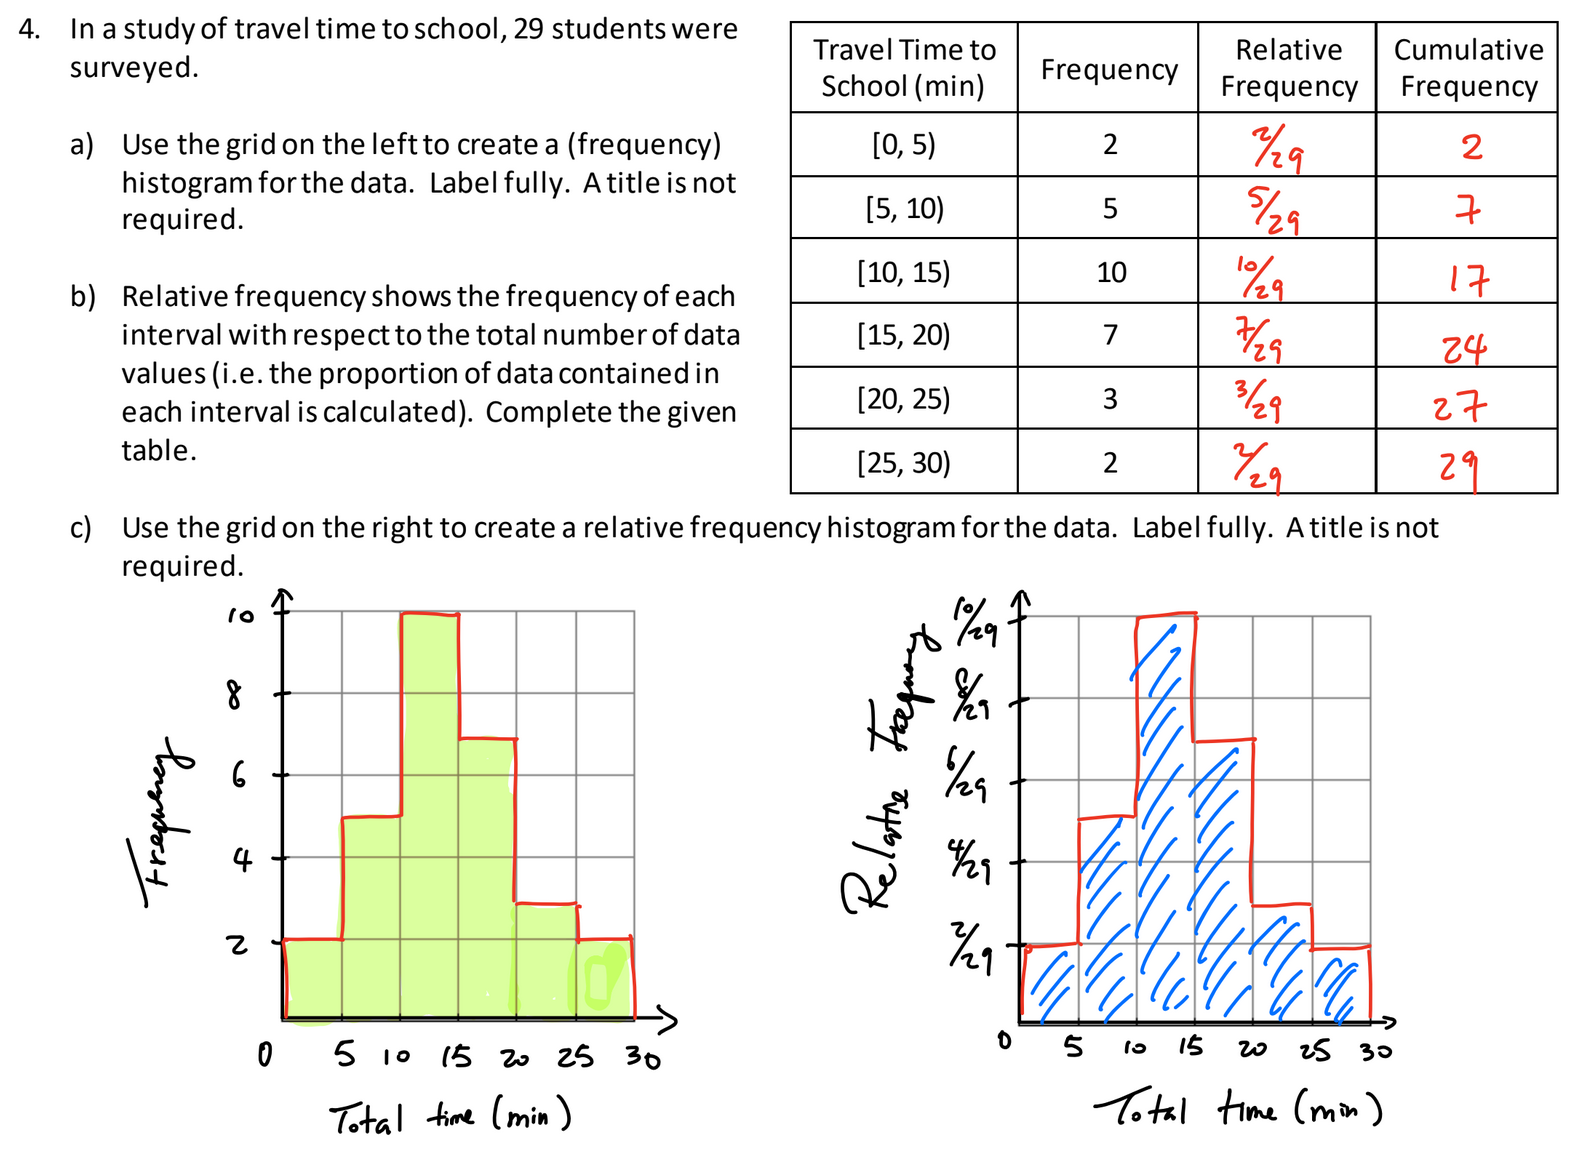
\includegraphics[width=0.8\textwidth]{pictures/3.2.3.png}
\caption{Example}
\end{figure}

Like a histogram, a \textbf{frequency polygon} gives an idea of the shape of the data distribution. It helps show the changes
in frequency from one interval to the next. If the midpoint of each interval is used as an estimate for the all the values in the 
interval, then a frequency polygon is a line graph joining the mindpoints of the top of adjacent bars of a histogram. \\

Check the note\\

\section{Central Tendency}
\subsection{Definitions of Central Tendency}
\subsubsection{CENTRAL}
Measure of \textbf{CENTRAL} tendency are used to determine the averages of a set of data\\

\subsubsection{Mean}
The \textbf{Mean} of a set of numerical data is equal to the sum of the values of a variable divided by the number 
of values. That is:
\begin{equation*}
    \text{population mean} = \mu = \frac{x_1 + x_2 + \cdots + x_N}{N} = \frac{\sum_{i = 1}^{N} x_i}{N}
\end{equation*}

\begin{equation*}
    \text{sample mean} = \bar{x} = \frac{x_1 + x_2 + \cdots + x_n}{n} = \frac{\sum_{i = 1}^{n} x_i}{n}
\end{equation*}

If a set of numerical data is listed from least to greatest, then:
\begin{enumerate}
    \item the median is the middle number (or the mean of the Two middle numbers), and,
    \item the values can be ranked such that the minimum has rank=1 and the maximum has rank = N or n
\end{enumerate}

The \textbf{Mode} is the most frequently occurred value in the data\\

The \textbf{MODAL} interval is the interval that contains the msot number of values\\

\textbf{OUTLIERS} are values that are significantly distant from the majority of the data

\subsubsection{How to choose form}
\begin{enumerate}
    \item If the data is \textbf{not} numeric, use the Mode
    \item if the data contain outliers and/or mean is skewed, use the median
    \item otherwise use the mean
\end{enumerate}
\subsubsection{Weighted}
the Weighted mean reflects the relative importance of each value of the data set. They could be calculated by two formulas:\\

Population:
\[
    \mu_w = \frac{w_1x_1 + w_2x_2 + \cdots + w_Nx_N}{w_1 + w_2 + \cdots + w_N} = \frac{\sum_{i = 1}^{N} w_ix_i}{\sum_{i = 1}^{N}w_i}
\]

Sample:
\[
    \bar{x}_w = \frac{w_1x_1 + w_2x_2 + \cdots + w_Nx_N}{w_1 + w_2 + \cdots + w_N} = \frac{\sum_{i = 1}^{n} w_ix_i}{\sum_{i = 1}^{n}w_i}
\]

\section{Standard Deviation}
\subsubsection{Spread}
Measures of \tbf{spread} are frequently calculated when analyzing numerical data. These measures are values that quantify how 
consistent or spread out of a set of data is. A measure of spread is often used to determine which of serval sets of data is 
more consistent\\

The \tbf{spread} of a set of data is \tbf{zero} if all the values in the set are identical\\

Just as there are several measures of central tendency, there are \tbf{several} different measures of spread. Variance and 
standard deviation are two of these measures.\\

The \tbf{Deviation} of a piece of data is the difference between the value of that piece of data and the mean of the set

\subsubsection{Deviation of Detum}
Population:
\[
    x - \mu
\]

Sample:
\[
    x - \bar{x}
\]

\begin{definition}
    Variance: The mean of the squares of the deviations. Larger variance = spread of the data is larger
\end{definition}
Population Variance:
\[
    \sigma^s = \frac{\sum (x - \mu)^2}{N}
\]

Sample variance:
\[
    s^2 = \frac{\sum (x - \bar{x})^2}{n - 1}
\]

Sample variance's denominator being $n-1$ as opposed to $n$ because in a sample the deviations tend to be underestimated.

\subsubsection{Standard deviation}
\begin{definition}
    Standard Deviation approximates the \tbf{TYPICAL} distance from the mean to each datum in the set
\end{definition}
Population standard deviation:
\begin{equation*}
    \sigma = \sqrt{\frac{\sum (x - \mu)^2}{N}}
\end{equation*}
Sample standard deviation:
\begin{equation*}
    s = \sqrt{\frac{\sum (x - \bar{x})^2}{n - 1}}
\end{equation*}

\begin{remark}
    Always calculate the sample variance/standard deviation if it is not clear whether the data is from a census or from a sample
\end{remark}

\subsubsection{Z-score}
A datum's z-score is the \red{number} of standard deviations that datum is above or below the mean of the data set. Hence:\\
\begin{gather*}
    z = \frac{x - \mu}{\sigma}\\
    z = \frac{x - \bar{x}}{s}
\end{gather*}

\section{Quartiles}
\subsection{Definitions}
\begin{definition}
    Interquartiles range is the measures of spread
\end{definition}
\subsubsection{Range}
Range is the difference between the largest and smallest values and it does not give any information about the spread of the other data values
in the set 

\subsubsection{Quartiles}
Quartiles divide a set of ordered data into 4 equal groups, similar to a median that divides the data into 2 
equal groups. The three dividers are the first quartile $Q_1$, the second quartile $Q_2$ and the third quartile
$Q_3$\\

$Q_2$ can be seen as the median of a data set. $Q_1$ and $Q_3$ can be defined as the \tbf{Median} of the lower and upper
halves of the set, respectively, with an understanding of that, if the ordered set has an odd number of values then the
middle number is not part of the lower or upper half of the data set

\subsubsection{InterQuartile}
It is the range of the middle half of the data. It can be calculated by this formula:
\[
    IQR = Q_3 - Q_1
\]

A larger $IQE$ indicates a greater spread of the central half of the data. The \tbf{semi-interquartile} range is the 
$IQE$ divide by 2

\subsubsection{Box-and-whisker plots}
    This graph illustrate the spread of the data around the \tbf{MEDIAN}. The box shows three quartile values, a left and a 
right whisker that "lead" to the minimum and the maximum values of the data set

\mypic{pictures/3.4.1.png}{An example of box-and-whisker plot}{0.7}

\subsubsection{Outlier}
A \tbf{Modified} box plot may be used if the data contains outliers. Any value of $x$ that is at 
least 1.5 times the box length from the box are considered outliers. These outliers must be plot 
as separate points instead of including them as part of the whiskers
\begin{figure}[h!]
    \centering
    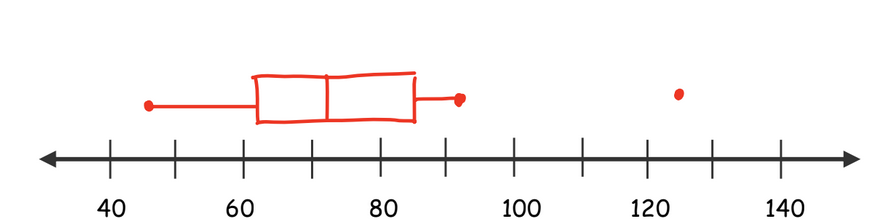
\includegraphics[width=0.5\textwidth]{pictures/3.4.1.2.png}
    \caption{In this graph, 125 is an example of outlier}
\end{figure}

\subsection{Percentiles}
\tbf{Percentiles} divide a set of data into 100 equal intervals. A common definition for percentiles states that 
"A value corresponds to the $k^{th}$ percentile if $k$ \% of the data are less than or equal to the value"\\

For a data set of n:\\

The Rank of the percentile p is:
\begin{equation*}
    R = \frac{p*n}{100}
\end{equation*}
Else linear interpolate the values with rank $R$ and $R + 1$ to determine the value that corresponds to percentile $p$

The percentile that corresponds to a specific datum is:
\begin{equation*}
    p = \frac{100L}{n}
\end{equation*}
\begin{center}
    $L$ is the number of data values less than or equal to that specific datum
\end{center}

\subsubsection{\red{Remainder}}
$Q_1$ and the $25^{th}$ percentile corresponds to the same location of the data set, two \red{different}
methods are being used to find the two statistics, for the purpose of convenience. Hence, they may not 
be equal to each other even though they should.

\section{Spread Grouped Data}
\subsection{For weighted data}
If $x_i$ represents the $i^{th}$ distinct value and $w_i$ represents the weighting of the value $x_i$ them\\

Average:
\begin{equation}
    M \text{ or } x_i = \frac{\sum (w_i * x_i)}{N}
\end{equation}

Population deviation:
\begin{equation}
    \sigma = \sqrt{\frac{\sum w_i * (x_i - M)}{N}}
\end{equation}

For sample deviation:
\begin{equation}
    s = \sqrt{\frac{\sum w_i * (x_i - \bar{x})}{n - 1}}
\end{equation}

\section{Collect data}
\subsection{Anonymous and not be anonymous}
\begin{definition}
    (Anonymous): More likely to get honest data (hence more reliable data)
\end{definition}
\begin{definition}
    (Not Anonymous): Show credibility of Survey (answers)
\end{definition}

\subsection{Survey Questions}
\subsubsection*{Open}
Respondents answer in their own words

\subsubsection*{Closed}
\begin{definition}
    (checklist): Choose as many as apply (With a rating scale should be evenly distributed)
\end{definition}
\begin{definition}
    (Ranking): Give a rank based on the choices
\end{definition}

\subsection{Questions should be avoided}
\begin{definition}
    (Double-Barrelled): A question that akss more than one topic. (Ex. Do you like Math and Science?)
\end{definition}
\begin{definition}
    (Leading Question): Encourages a particular answer, onften becauses of this question is phrased or presented
\end{definition}
\begin{definition}
    (Loaded Question): A question contains assumptions, where answering it means the respondent accepts what the questioner is assuming
\end{definition}

\subsection{Experimental vs Observational study}
\subsubsection*{Observational study}
\begin{itemize}
    \item Study about how one factor affect another factor, without make any \red{attempt to intervene}
\end{itemize}

\subsubsection*{Experimental study}
\begin{itemize}
    \item Try to determine the cause and effect relationship between two variables by changing the 
    value or characteristics of one variable to see what effect it has on the other variable
    \item Randomly place participants into the experimental group and the control group, with each group having a similar demographic make-up
    \item One experimental(Treatment) group of an experimental study receive the specific Treatment
    \item The other one do not receive the specific treatment being measured
\end{itemize}

\section{sampling}
\begin{definition}
    (Population): referss to the entire group that is being studied. Also called descriptive statistics
\end{definition}
\begin{definition}
    (Sample): Is a portion of the population. Summary values calculated from the sample data are called statistics. 
    The term \red{inferential statistics} describes the process of generalizing about the population based on 
    sample data. Therefore, it is important to have a "representative sample" when performing a statistical study
\end{definition}

\subsection{Some type of sampling}
\begin{definition}
    (Simple Random Sampling): every member of the population has an \red{equal chance} of being chosen for the study.
\end{definition}

\begin{definition}
    (SYSTEMIC Random Sampling): Individuals are selected at regular intervals, starting with a randomly chosen position.
\end{definition}

\begin{definition}
    (Stratified Random Sampling): Population is divied into groups/strata such that all members in each stratum share common
    characteristics but are different from members in other strata, then the same \underline{proportion} of members from each 
    stratum are randomly chosen 
\end{definition}

\begin{definition}
    (Cluster random sampling): The population is divied into groups/clusters such that each cluster is a 
    representative of the whole population, then every member of a random sample cluster are are surveyed
\end{definition}

\begin{definition}
    (Multi-stage random sampling): more than one loevel of random sampling techniques are applied
\end{definition}

\begin{definition}
    (Voluntary-response random sampling): members of the population are invited to participate in the survey and 
    anyone who choose to participate is the sample
\end{definition}

\begin{definition}
    (Voluntary-response random sampling): members of the population are invited to participate in the survey and 
    anyone who choose to participate is the sample
\end{definition}

\begin{definition}
    (Convenience random sampling): the sample is selected because it is easily accesible. 
\end{definition}

\section{Bias}
\begin{definition}
    (Sampling bias): When the sample is not representative of the population
\end{definition}
\begin{definition}
    (Measurement bias): the data measuring tools are poorly designed
\end{definition}
\begin{definition}
    (Response bias): when participants in a survey deliberately give false or misleading answers
\end{definition}
\begin{definition}
    (Non-response bias): a form of sampling bias, particular groups are under-represented because they choose not to participate
\end{definition}